\documentclass[11pt, a4paper]{article}

\usepackage{fontspec}
\usepackage{unicode-math}
\setmainfont{texgyrepagella-regular.otf}[
    Path = fonts/,
    BoldFont = texgyrepagella-bold.otf,
    ItalicFont = texgyrepagella-italic.otf,
    BoldItalicFont = texgyrepagella-bolditalic.otf
]
\setmathfont{texgyrepagella-math.otf}[Path = fonts/]
\renewcommand{\boldsymbol}[1]{\symbf{#1}}
\usepackage{amsmath}

\newfontfamily\treefont{Consolas}

\usepackage[a4paper, margin=2cm, top=2cm, bottom=2cm]{geometry}
\usepackage{microtype}
\usepackage{titlesec}
\usepackage{tikz}

\linespread{1.05}
\setlength{\parindent}{0pt}
\setlength{\parskip}{2.5pt plus 1pt minus 0.5pt}

% Khoảng cách phương trình hiển thị
\setlength{\abovedisplayskip}{3pt plus 1pt minus 1pt}
\setlength{\belowdisplayskip}{3pt plus 1pt minus 1pt}

% Tiêu đề chương chuẩn academic
\titleformat{\section}
  {\large\bfseries}
  {\thesection}{0.5em}{}
\titlespacing*{\section}
  {0pt}{14pt plus 3pt minus 2pt}{6pt plus 1pt minus 1pt}

% Lệnh dựng nút và đường nhánh cây (Tree node)
\newdimen\trw
\newcommand{\TrNode}[2]{%
  \noindent\settowidth{\trw}{{\treefont #1\ }}%
  \hangindent=\trw \hangafter=1
  {\treefont #1\ }#2\par
}
\newcommand{\TrLine}[1]{\noindent{\treefont #1}\par}

\pagestyle{plain}

\begin{document}

%=====================================================================
% TRANG 1: SƠ ĐỒ CÂY TỔNG QUAN (TOPIC TREE MAP THEO CHUẨN CSTSL)
%=====================================================================
\begin{center}
    {\Large\bfseries MINDMAP VLĐT}
\end{center}
\vspace{0.6cm}

\noindent
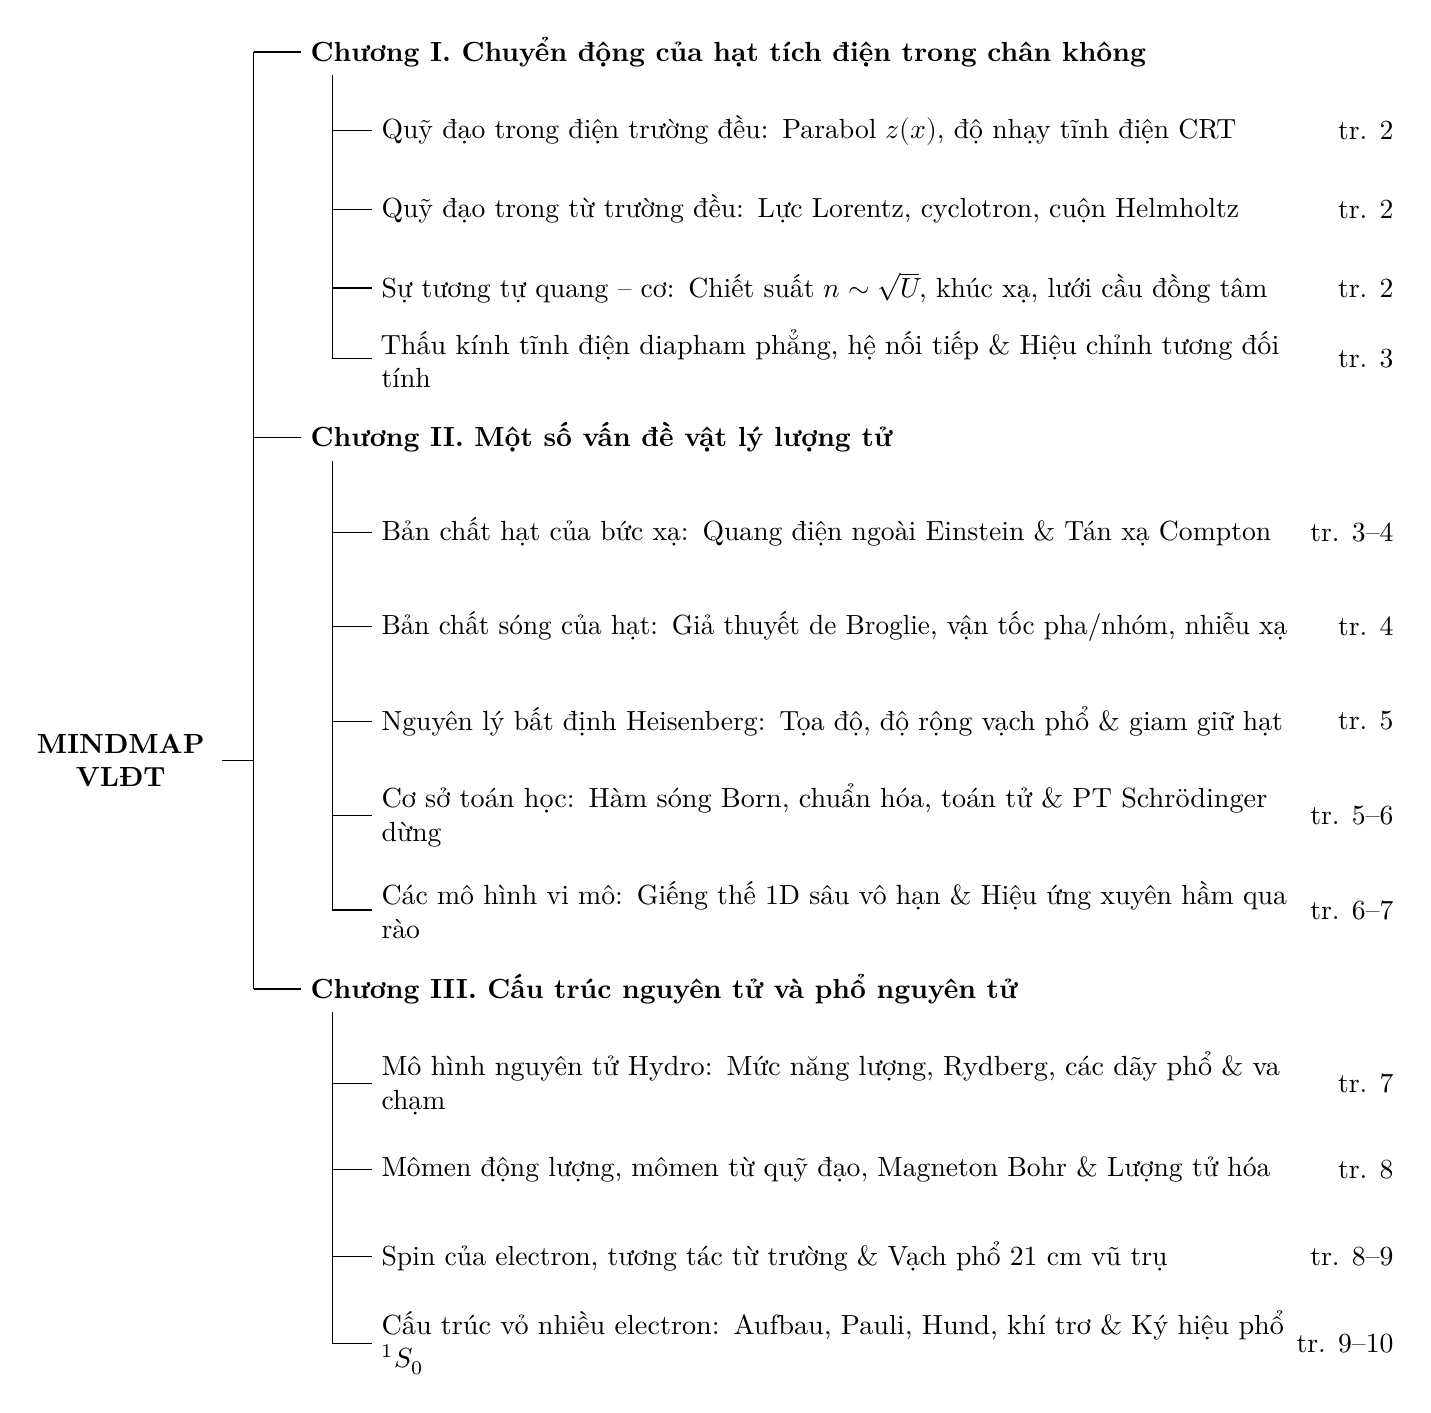
\begin{tikzpicture}[x=1mm, y=1mm]
  \def\spineX{24}
  \def\groupX{30}
  \def\subspineX{34}
  \def\leafX{39}
  \def\rightX{170}

  \coordinate (root) at (20, 115);

  % Toạ độ dọc y các chương
  \def\yChI{205}
  \def\yChIe{166}

  \def\yChII{156}
  \def\yChIIe{96}

  \def\yChIII{86}
  \def\yChIIIe{41}

  % Khung gốc và trục chính (Main spine)
  \draw[line width=0.6pt] (root) -- (\spineX, 115);
  \node[anchor=east, align=center, font=\bfseries] at (19, 115) {MINDMAP\\VLĐT};
  \draw[line width=0.6pt] (\spineX, \yChI) -- (\spineX, \yChIII);

  % --- CHƯƠNG I ---
  \draw[line width=0.6pt] (\spineX, \yChI) -- (\groupX, \yChI);
  \node[anchor=west, font=\bfseries] at (\groupX, \yChI) {Chương I. Chuyển động của hạt tích điện trong chân không};

  \draw[line width=0.4pt] (\subspineX, \yChI - 3) -- (\subspineX, \yChIe);

  \draw[line width=0.4pt] (\subspineX, 195) -- (\leafX, 195);
  \node[anchor=west, text width=115mm] at (\leafX, 195) {Quỹ đạo trong điện trường đều: Parabol $z(x)$, độ nhạy tĩnh điện CRT};
  \node[anchor=east] at (\rightX, 195) {tr. 2};

  \draw[line width=0.4pt] (\subspineX, 185) -- (\leafX, 185);
  \node[anchor=west, text width=115mm] at (\leafX, 185) {Quỹ đạo trong từ trường đều: Lực Lorentz, cyclotron, cuộn Helmholtz};
  \node[anchor=east] at (\rightX, 185) {tr. 2};

  \draw[line width=0.4pt] (\subspineX, 175) -- (\leafX, 175);
  \node[anchor=west, text width=115mm] at (\leafX, 175) {Sự tương tự quang -- cơ: Chiết suất $n \sim \sqrt{U}$, khúc xạ, lưới cầu đồng tâm};
  \node[anchor=east] at (\rightX, 175) {tr. 2};

  \draw[line width=0.4pt] (\subspineX, 166) -- (\leafX, 166);
  \node[anchor=west, text width=115mm] at (\leafX, 166) {Thấu kính tĩnh điện diapham phẳng, hệ nối tiếp \& Hiệu chỉnh tương đối tính};
  \node[anchor=east] at (\rightX, 166) {tr. 3};

  % --- CHƯƠNG II ---
  \draw[line width=0.6pt] (\spineX, \yChII) -- (\groupX, \yChII);
  \node[anchor=west, font=\bfseries] at (\groupX, \yChII) {Chương II. Một số vấn đề vật lý lượng tử};

  \draw[line width=0.4pt] (\subspineX, \yChII - 3) -- (\subspineX, \yChIIe);

  \draw[line width=0.4pt] (\subspineX, 144) -- (\leafX, 144);
  \node[anchor=west, text width=115mm] at (\leafX, 144) {Bản chất hạt của bức xạ: Quang điện ngoài Einstein \& Tán xạ Compton};
  \node[anchor=east] at (\rightX, 144) {tr. 3--4};

  \draw[line width=0.4pt] (\subspineX, 132) -- (\leafX, 132);
  \node[anchor=west, text width=115mm] at (\leafX, 132) {Bản chất sóng của hạt: Giả thuyết de Broglie, vận tốc pha/nhóm, nhiễu xạ};
  \node[anchor=east] at (\rightX, 132) {tr. 4};

  \draw[line width=0.4pt] (\subspineX, 120) -- (\leafX, 120);
  \node[anchor=west, text width=115mm] at (\leafX, 120) {Nguyên lý bất định Heisenberg: Tọa độ, độ rộng vạch phổ \& giam giữ hạt};
  \node[anchor=east] at (\rightX, 120) {tr. 5};

  \draw[line width=0.4pt] (\subspineX, 108) -- (\leafX, 108);
  \node[anchor=west, text width=115mm] at (\leafX, 108) {Cơ sở toán học: Hàm sóng Born, chuẩn hóa, toán tử \& PT Schrödinger dừng};
  \node[anchor=east] at (\rightX, 108) {tr. 5--6};

  \draw[line width=0.4pt] (\subspineX, 96) -- (\leafX, 96);
  \node[anchor=west, text width=115mm] at (\leafX, 96) {Các mô hình vi mô: Giếng thế 1D sâu vô hạn \& Hiệu ứng xuyên hầm qua rào};
  \node[anchor=east] at (\rightX, 96) {tr. 6--7};

  % --- CHƯƠNG III ---
  \draw[line width=0.6pt] (\spineX, \yChIII) -- (\groupX, \yChIII);
  \node[anchor=west, font=\bfseries] at (\groupX, \yChIII) {Chương III. Cấu trúc nguyên tử và phổ nguyên tử};

  \draw[line width=0.4pt] (\subspineX, \yChIII - 3) -- (\subspineX, \yChIIIe);

  \draw[line width=0.4pt] (\subspineX, 74) -- (\leafX, 74);
  \node[anchor=west, text width=115mm] at (\leafX, 74) {Mô hình nguyên tử Hydro: Mức năng lượng, Rydberg, các dãy phổ \& va chạm};
  \node[anchor=east] at (\rightX, 74) {tr. 7};

  \draw[line width=0.4pt] (\subspineX, 63) -- (\leafX, 63);
  \node[anchor=west, text width=115mm] at (\leafX, 63) {Mômen động lượng, mômen từ quỹ đạo, Magneton Bohr \& Lượng tử hóa};
  \node[anchor=east] at (\rightX, 63) {tr. 8};

  \draw[line width=0.4pt] (\subspineX, 52) -- (\leafX, 52);
  \node[anchor=west, text width=115mm] at (\leafX, 52) {Spin của electron, tương tác từ trường \& Vạch phổ 21 cm vũ trụ};
  \node[anchor=east] at (\rightX, 52) {tr. 8--9};

  \draw[line width=0.4pt] (\subspineX, 41) -- (\leafX, 41);
  \node[anchor=west, text width=115mm] at (\leafX, 41) {Cấu trúc vỏ nhiều electron: Aufbau, Pauli, Hund, khí trơ \& Ký hiệu phổ $^1S_0$};
  \node[anchor=east] at (\rightX, 41) {tr. 9--10};

\end{tikzpicture}

\newpage

%=====================================================================
% TRANG 2 TRỞ ĐI: NỘI DUNG CHI TIẾT TỪNG CHƯƠNG DẠNG TREE
%=====================================================================

%=====================================================================
% CHƯƠNG I
%=====================================================================
\section*{Chương I. Chuyển động của hạt tích điện trong chân không}

\TrLine{│}
\TrNode{├──}{\textbf{1. QUỸ ĐẠO CỦA ĐIỆN TỬ TRONG ĐIỆN TRƯỜNG ĐỀU ($\vec{E} = \text{const}$)}}
\TrLine{│   │}
\TrNode{│   ├──}{\textbf{1.1. Phương trình chuyển động và quỹ đạo parabol}}
\TrNode{│   │   ├──}{Gia tốc hướng dọc theo điện trường: $\vec{a} = -\dfrac{e}{m}\vec{E} \implies a_z = \dfrac{e E}{m} = \dfrac{e U_k}{m d}$}
\TrNode{│   │   ├──}{Vận tốc ban đầu của electron sau khi được tăng tốc qua hiệu điện thế $U_0$: $v_0 = \sqrt{\dfrac{2eU_0}{m}}$}
\TrNode{│   │   └──}{Phương trình quỹ đạo trong bản lái tia phẳng dài $l_1$, cách nhau $d$: Parabol $z(x) = \dfrac{e U_k}{2 m d v_0^2} x^2 = \dfrac{U_k}{4 d U_0} x^2$ ($0 \le x \le l_1$)}
\TrLine{│   │}
\TrNode{│   └──}{\textbf{1.2. Độ lệch chùm tia \& Độ nhạy tĩnh điện của ống CRT [Bài 1-1]}}
\TrNode{│       ├──}{Khoảng cách từ điểm giữa hai bản lái tia đến màn huỳnh quang: $L = \dfrac{l_1}{2} + l_2$}
\TrNode{│       ├──}{Độ lệch của vết sáng trên màn huỳnh quang: $D = z(l_1) + \left.\dfrac{dz}{dx}\right|_{l_1} l_2 = \dfrac{U_k l_1 L}{2 d U_0}$}
\TrNode{│       ├──}{Độ nhạy tĩnh điện của ống phóng điện tử: $S_E = \dfrac{|D|}{U_k} = \dfrac{l_1 L}{2 d U_0}$ (đơn vị: mm/V hay m/V)}
\TrNode{│       └──}{\textit{[Bài tập áp dụng: Bài 1-1]}}
\TrLine{│}
\TrNode{├──}{\textbf{2. QUỸ ĐẠO CỦA ĐIỆN TỬ TRONG TỪ TRƯỜNG ĐỀU ($\vec{B} = \text{const}$)}}
\TrLine{│   │}
\TrNode{│   ├──}{\textbf{2.1. Lực từ Lorentz và chuyển động Cyclotron ($\vec{v}_0 \perp \vec{B}$)}}
\TrNode{│   │   ├──}{Lực Lorentz đóng vai trò lực hướng tâm: $F_L = e v_0 B = \dfrac{m v_0^2}{R}$}
\TrNode{│   │   ├──}{Bán kính quỹ đạo tròn: $R = \dfrac{m v_0}{e B} = \dfrac{\sqrt{2 m e U_0}}{e B} = \dfrac{1}{B}\sqrt{\dfrac{2m U_0}{e}}$}
\TrNode{│   │   └──}{Chu kỳ, tần số và tần số góc cyclotron: $T = \dfrac{2\pi m}{e B}, \quad f = \dfrac{e B}{2\pi m}, \quad \omega = \dfrac{e B}{m}$ (không phụ thuộc bán kính $R$ và vận tốc $v_0$)}
\TrLine{│   │}
\TrNode{│   └──}{\textbf{2.2. Độ lệch từ trường \& Hệ cuộn dây Helmholtz [Bài 1-2]}}
\TrNode{│       ├──}{Chùm tia qua vùng từ trường hẹp bề rộng $l_1$ ($R \gg l_1$): Quỹ đạo gần đúng là cung parabol}
\TrNode{│       ├──}{Độ lệch trên màn huỳnh quang: $D \approx \theta L \approx \dfrac{l_1}{R} L = \sqrt{\dfrac{e}{2 m U_0}} B l_1 L$}
\TrNode{│       ├──}{Từ trường trục cặp cuộn dây Helmholtz ($W$ vòng mỗi cuộn, bán kính $R_H$, cách nhau $R_H$): $B = \dfrac{8 \mu_0 W I}{5\sqrt{5} R_H}$}
\TrNode{│       ├──}{Độ nhạy từ trường: $S_M = \dfrac{D}{I} = \sqrt{\dfrac{e}{2 m U_0}} l_1 L \dfrac{B}{I}$ (đơn vị: mm/A)}
\TrNode{│       └──}{\textit{[Bài tập áp dụng: Bài 1-2]}}
\TrLine{│}
\TrNode{├──}{\textbf{3. SỰ TƯƠNG TỰ QUANG -- CƠ (QUANG HỌC ĐIỆN TỬ)}}
\TrLine{│   │}
\TrNode{│   ├──}{\textbf{3.1. Hệ thức tương đương giữa chiết suất và điện thế}}
\TrNode{│   │   ├──}{Hệ thức tương đương: $n \sim v \sim \sqrt{U}$}
\TrNode{│   │   ├──}{Định luật khúc xạ quang học điện tử: $\dfrac{\sin\alpha}{\sin\beta} = \dfrac{v_2}{v_1} = \sqrt{\dfrac{U_2}{U_1}}$ ($\alpha$: góc tới; $\beta$: góc khúc xạ)}
\TrNode{│   │   ├──}{Điều kiện phản xạ toàn phần ($U_2 < U_1$): $\sin\alpha \ge \sin\alpha_{gh} = \sqrt{\dfrac{U_2}{U_1}}$}
\TrNode{│   │   └──}{Điều kiện để electron rơi trên mặt kim loại có thế hãm $U_{\text{KL}}$: $\sin\alpha \le \sqrt{1 - \dfrac{U_{\text{KL}}}{U_0}}$}
\TrLine{│   │}
\TrNode{│   └──}{\textbf{3.2. Mặt cầu đẳng thế và hệ lưới cầu đồng tâm [Bài 1-3]}}
\TrNode{│       ├──}{Khúc xạ qua mặt cầu đẳng thế bán kính $R$: $\dfrac{n_2}{f_2} = \dfrac{n_1}{f_1} = \dfrac{n_2 - n_1}{R}$}
\TrNode{│       ├──}{Tiêu cự đối xứng: $f_1 = \dfrac{\sqrt{U_1}}{\sqrt{U_2} - \sqrt{U_1}} R, \quad f_2 = \dfrac{\sqrt{U_2}}{\sqrt{U_2} - \sqrt{U_1}} R$}
\TrNode{│       ├──}{Chứng minh tính hội tụ: Với $U_2 > U_1 \implies f_1, f_2 > 0$, hệ luôn có tính hội tụ đối với chùm điện tử}
\TrNode{│       └──}{\textit{[Bài tập áp dụng: Bài 1-3]}}
\TrLine{│}
\TrNode{└──}{\textbf{4. THẤU KÍNH TĨNH ĐIỆN VÀ HIỆU CHỈNH TƯƠNG ĐỐI TÍNH}}
\TrNode{    ├──}{\textbf{4.1. Thấu kính một màng chắn phẳng (Diapham) [Bài 1-4]}}
\TrNode{    │   ├──}{Tiêu cự của diapham điện thế $U_D$: $f = \dfrac{4 U_D}{E_2 - E_1}$}
\TrNode{    │   ├──}{Điện trường hai phía: $E_1 = \dfrac{U_D - U_G}{d_1}$ (lưới $G$ tới $D$), $E_2 = \dfrac{U_A - U_D}{d_2}$ ($D$ tới anot $A$)}
\TrNode{    │   ├──}{$E_2 - E_1 > 0 \implies f > 0$: Thấu kính có tính hội tụ}
\TrNode{    │   ├──}{$E_2 - E_1 < 0 \implies f < 0$: Thấu kính có tính phân kỳ}
\TrNode{    │   ├──}{Điều kiện chùm electron song song hội tụ đúng lên anot: Tiêu cự $f = d_2$}
\TrNode{    │   └──}{\textit{[Bài tập áp dụng: Bài 1-4]}}
\TrNode{    ├──}{\textbf{4.2. Hệ thấu kính tĩnh điện nối tiếp [Bài 1-5]}}
\TrNode{    │   ├──}{Công thức thấu kính mỏng (Gauss): $\dfrac{1}{f} = \dfrac{1}{d} + \dfrac{1}{d'}$}
\TrNode{    │   ├──}{Ghép hai thấu kính đồng trục cách nhau khoảng $L$: $d_2 = L - d_1'$}
\TrNode{    │   └──}{\textit{[Bài tập áp dụng: Bài 1-5]}}
\TrNode{    └──}{\textbf{4.3. Hiệu chỉnh tương đối tính khi vận tốc tiệm cận tốc độ ánh sáng ($v \to c$)}}
\TrNode{        ├──}{Khối lượng tương đối tính: $m = \gamma m_0 = \dfrac{m_0}{\sqrt{1 - v^2/c^2}}$}
\TrNode{        ├──}{Vận tốc electron gia tốc qua hiệu điện thế $U$: $v = c\sqrt{1 - \dfrac{1}{\left(1 + \dfrac{eU}{m_0 c^2}\right)^2}}$}
\TrNode{        └──}{Chiết suất hiệu dụng tương đối tính: $n \propto \sqrt{U\left(1 + \dfrac{eU}{2m_0 c^2}\right)}$}

\vspace{0.4cm}

%=====================================================================
% CHƯƠNG II
%=====================================================================
\section*{Chương II. Một số vấn đề vật lý lượng tử}

\TrLine{│}
\TrNode{├──}{\textbf{1. BẢN CHẤT HẠT CỦA BỨC XẠ ĐIỆN TỪ (THUYẾT PHOTON)}}
\TrLine{│   │}
\TrNode{│   ├──}{\textbf{1.1. Khủng hoảng của cơ học/sóng cổ điển}}
\TrNode{│   │   ├──}{Khái niệm photon: Lượng tử mang năng lượng $E_\gamma = h\nu = \hbar\omega = \dfrac{hc}{\lambda}$, động lượng $p = \dfrac{h}{\lambda} = \dfrac{E}{c}$, khối lượng nghỉ $m_0 = 0$}
\TrNode{│   │   ├──}{Mô hình sóng cổ điển: Nguyên tử hấp thụ bức xạ liên tục theo thời gian, năng lượng phân bố đều trên mặt cầu}
\TrNode{│   │   ├──}{Cường độ phát xạ đẳng hướng tại khoảng cách $R$: $I = \dfrac{P_{\text{bx}}}{4\pi R^2}$}
\TrNode{│   │   ├──}{Công suất nguyên tử tiết diện đĩa $S_a = \dfrac{\pi d^2}{4}$ hứng được: $P_a = I \cdot S_a = \dfrac{P_{\text{bx}} d^2}{16 R^2}$}
\TrNode{│   │   ├──}{Thời gian tích lũy công thoát $\varphi$: $t = \dfrac{\varphi}{P_a} = \dfrac{16 R^2 \varphi}{P_{\text{bx}} d^2}$}
\TrNode{│   │   └──}{Mâu thuẫn thực nghiệm: $t_{\text{cổ điển}} \sim 58\text{ s}$ trong khi thực tế quang điện xảy ra tức thời ($< 10^{-9}\text{ s}$)}
\TrNode{│   │       └──}{\textit{[Bài tập áp dụng: Bài 2-1]}}
\TrLine{│   │}
\TrNode{│   ├──}{\textbf{1.2. Hiện tượng quang điện ngoài \& Thuyết photon Einstein}}
\TrNode{│   │   ├──}{Phương trình Einstein: $h\nu = \dfrac{hc}{\lambda} = \varphi + W_{\text{đ}\max} = \varphi + \dfrac{1}{2}m v_{0\max}^2$}
\TrNode{│   │   ├──}{Động năng ban đầu cực đại \& Thế hãm: $W_{\text{đ}\max} = e U_h = \dfrac{hc}{\lambda} - \varphi$}
\TrNode{│   │   ├──}{Giới hạn quang điện (bước sóng ngưỡng): $\lambda_0 = \dfrac{hc}{\varphi}$ (điều kiện xảy ra quang điện: $\lambda \le \lambda_0$ hay $\nu \ge \nu_0$)}
\TrNode{│   │   └──}{Thông lượng photon và dòng quang điện: $\Phi_\gamma = \dfrac{I}{E_\gamma} = \dfrac{I\lambda}{hc}$ (với hiệu suất $\eta$: $n_e = \eta \Phi_\gamma$)}
\TrNode{│   │       └──}{\textit{[Bài tập áp dụng: Bài 2-2]}}
\TrLine{│   │}
\TrNode{│   └──}{\textbf{1.3. Hiệu ứng Compton (Tán xạ photon trên electron tự do)}}
\TrNode{│       ├──}{Bản chất: Va chạm đàn hồi giữa photon tia X và electron tự do ban đầu đứng yên ($v_0 = 0$)}
\TrNode{│       ├──}{Định luật bảo toàn năng lượng toàn phần và xung lượng tương đối tính:}
\TrNode{│       │   ├──}{Bảo toàn năng lượng: $\dfrac{hc}{\lambda} + m_0 c^2 = \dfrac{hc}{\lambda'} + mc^2 = \dfrac{hc}{\lambda'} + \sqrt{p_e^2 c^2 + m_0^2 c^4}$}
\TrNode{│       │   └──}{Bảo toàn động lượng vectơ: $\vec{p}_\gamma = \vec{p}'_\gamma + \vec{p}_e \implies p_e^2 = p_\gamma^2 + {p'}_\gamma^2 - 2 p_\gamma p'_\gamma \cos\theta$}
\TrNode{│       ├──}{Công thức tán xạ Compton: $\Delta\lambda = \lambda' - \lambda = \lambda_C(1 - \cos\theta) = 2\lambda_C \sin^2(\theta/2)$}
\TrNode{│       │   └──}{Bước sóng Compton của electron: $\lambda_C = \dfrac{h}{m_0 c} \approx 0{,}02426\text{ \AA} = 2{,}426 \cdot 10^{-12}\text{ m}$}
\TrNode{│       └──}{Động năng \& Vận tốc giật lùi của electron:}
\TrNode{│           ├──}{Động năng electron nhận: $W_{\text{đ}e} = E_\gamma - E'_\gamma = hc\left(\dfrac{1}{\lambda} - \dfrac{1}{\lambda'}\right)$}
\TrNode{│           └──}{Vận tốc tương đối tính: $\gamma = 1 + \dfrac{W_{\text{đ}e}}{m_0 c^2} \implies v_e = c\sqrt{1 - \dfrac{1}{\gamma^2}}$}
\TrNode{│           └──}{\textit{[Bài tập áp dụng: Bài 2-3]}}
\TrLine{│}
\TrNode{├──}{\textbf{2. BẢN CHẤT SÓNG CỦA HẠT VẬT CHẤT (SÓNG DE BROGLIE)}}
\TrLine{│   │}
\TrNode{│   ├──}{\textbf{2.1. Giả thuyết de Broglie \& Hệ thức bước sóng}}
\TrNode{│   │   ├──}{Công thức tổng quát cho mọi hạt: $\lambda = \dfrac{h}{p}$}
\TrNode{│   │   ├──}{Hạt phi tương đối tính gia tốc qua thế $U$ ($W_{\text{đ}} = eU \ll m_0 c^2$): $p = \sqrt{2m_0 e U} \implies \lambda = \dfrac{h}{\sqrt{2m_0 e U}} \approx \dfrac{12{,}27}{\sqrt{U\text{ (V)}}}\text{ (\AA)}$}
\TrNode{│   │   │   └──}{\textit{[Bài tập áp dụng: Bài 2-4]}}
\TrNode{│   │   └──}{Hạt siêu tương đối tính ($W_{\text{đ}} \gg m_0 c^2$): $E^2 = p^2 c^2 + m_0^2 c^4 \implies pc \approx E \implies \lambda \approx \dfrac{hc}{E}$ (tiệm cận bước sóng photon)}
\TrNode{│   │       └──}{\textit{[Bài tập áp dụng: Bài 2-5]}}
\TrLine{│   │}
\TrNode{│   ├──}{\textbf{2.2. Vận tốc pha (Phase Velocity) và Vận tốc nhóm (Group Velocity)}}
\TrNode{│   │   ├──}{Vận tốc pha: $v_{\text{pha}} = \dfrac{\omega}{k} = \dfrac{E}{p}$}
\TrNode{│   │   │   ├──}{Dùng năng lượng toàn phần $E = mc^2$: $v_{\text{pha}} = \dfrac{c^2}{v} > c$ (không truyền tín hiệu)}
\TrNode{│   │   │   └──}{Dùng động năng cổ điển $E = mv^2/2$: $v_{\text{pha}} = \dfrac{v}{2}$}
\TrNode{│   │   └──}{Vận tốc nhóm: $v_g = \dfrac{d\omega}{dk} = \dfrac{dE}{dp} = v$ (trùng với vận tốc cơ học của hạt)}
\TrNode{│   │       └──}{\textit{[Bài tập áp dụng: Bài 2-6]}}
\TrLine{│   │}
\TrNode{│   └──}{\textbf{2.3. Bằng chứng thực nghiệm tính sóng của hạt}}
\TrNode{│       ├──}{Nhiễu xạ electron trên màng đa tinh thể (Định luật Bragg): $2d\sin\theta = n\lambda$ ($\theta$: góc trượt Bragg)}
\TrNode{│       │   └──}{Bán kính vân tròn trên màn cách $L$: $r = L\tan(2\theta) \approx 2L\theta \approx \dfrac{n L \lambda}{d}$}
\TrNode{│       │   └──}{\textit{[Bài tập áp dụng: Bài 2-7]}}
\TrNode{│       └──}{Giao thoa sóng vật chất qua hai khe Young: Khoảng vân $i = \dfrac{\lambda L}{d} = \dfrac{h L}{m v d}$}
\TrNode{│           └──}{\textit{[Bài tập áp dụng: Bài 2-8 (mô phỏng giả định $h$ lớn)]}}
\TrLine{│}
\TrNode{├──}{\textbf{3. NGUYÊN LÝ BẤT ĐỊNH HEISENBERG \& Ý NGHĨA VẬT LÝ}}
\TrLine{│   │}
\TrNode{│   ├──}{\textbf{3.1. Bất định Tọa độ -- Xung lượng ($x - p_x$)}}
\TrNode{│   │   ├──}{Hệ thức (giảng viên chốt): $\Delta x \cdot \Delta p_x \ge \dfrac{\hbar}{2} = \dfrac{h}{4\pi}$ (sách cũ dùng $\hbar$, đáp số gấp 2)}
\TrNode{│   │   ├──}{Đo độ chính xác phần nghìn: $\Delta p = 10^{-3}p$ (chú ý tính tương đối tính $p = \gamma mv$ khi $v$ lớn)}
\TrNode{│   │   │   └──}{\textit{[Bài tập áp dụng: Bài 2-9]}}
\TrNode{│   │   └──}{Trường hợp độ bất định bằng chính xung lượng ($\Delta p = p$): $\Delta x_{\min} = \dfrac{\hbar}{2p} = \dfrac{\lambda}{4\pi}$}
\TrNode{│   │       └──}{\textit{[Bài tập áp dụng: Bài 2-11]}}
\TrLine{│   │}
\TrNode{│   ├──}{\textbf{3.2. Bất định Năng lượng -- Thời gian ($E - t$)}}
\TrNode{│   │   ├──}{Hệ thức Heisenberg: $\Delta E \cdot \Delta t \ge \dfrac{\hbar}{2}$}
\TrNode{│   │   ├──}{Độ rộng tự nhiên vạch phổ \& Thời gian sống $\tau$ của mức kích thích: $\Delta E = h\Delta\nu = \dfrac{hc}{\lambda^2}\Delta\lambda \implies \tau = \dfrac{\hbar}{2\Delta E} = \dfrac{\lambda^2}{4\pi c \Delta\lambda}$}
\TrNode{│   │   │   └──}{\textit{[Bài tập áp dụng: Bài 2-10]}}
\TrNode{│   │   └──}{Chứng minh cơ học phi tương đối tính: $\Delta E = v\Delta p, \quad \Delta t = \dfrac{\Delta x}{v} \implies \Delta E \cdot \Delta t = \Delta p \cdot \Delta x \ge \dfrac{\hbar}{2}$}
\TrNode{│   │       └──}{\textit{[Bài tập áp dụng: Bài 2-12]}}
\TrLine{│   │}
\TrNode{│   └──}{\textbf{3.3. Hiện tượng giam giữ hạt (Confinement) \& Động năng tối thiểu}}
\TrNode{│       ├──}{Giam hạt trong kích thước $L$: $\Delta x = L$, $\Delta p = 2p \implies p_{\min} = \dfrac{\hbar}{4L} = \dfrac{h}{8\pi L}$}
\TrNode{│       ├──}{Động năng cực tiểu: $W_{\text{đ}\min} = \dfrac{p_{\min}^2}{2m} = \dfrac{h^2}{128\pi^2 mL^2}$ (hạt trong vùng giam giữ luôn có động năng điểm không khác 0)}
\TrNode{│       └──}{Bài toán electron trong hạt nhân ($L = 10^{-14}\text{ m}$): $pc \approx 4{,}9\text{ MeV} \gg m_0 c^2 \implies$ dùng TĐT, $W_{\text{đ}\min} \approx 4{,}45\text{ MeV} \gg$ thế liên kết $\implies$ Electron không thể ở trong hạt nhân}
\TrNode{│           └──}{\textit{[Bài tập áp dụng: Bài 2-13]}}
\TrLine{│}
\TrNode{├──}{\textbf{4. CƠ SỞ TOÁN HỌC CƠ HỌC LƯỢNG TỬ \& PHƯƠNG TRÌNH SCHRÖDINGER}}
\TrLine{│   │}
\TrNode{│   ├──}{\textbf{4.1. Hàm sóng \& Ý nghĩa thống kê Max Born}}
\TrNode{│   │   ├──}{Hàm sóng trạng thái $\Psi(x, t)$: Mô tả đầy đủ trạng thái vi mô}
\TrNode{│   │   ├──}{Mật độ xác suất tìm hạt: $W(x) = |\Psi(x, t)|^2 = \Psi^* \Psi$}
\TrNode{│   │   ├──}{Xác suất trong đoạn $[a, b]$: $P(a \le x \le b) = \displaystyle\int_a^b |\Psi(x)|^2 dx$}
\TrNode{│   │   └──}{Điều kiện chuẩn hóa toàn không gian: $\displaystyle\int_{-\infty}^{+\infty} |\Psi(x)|^2 dx = 1 \implies$ Biên độ hố thế $A = \sqrt{\dfrac{2}{L}}$}
\TrNode{│   │       └──}{\textit{[Bài tập áp dụng: Bài 2-17]}}
\TrLine{│   │}
\TrNode{│   ├──}{\textbf{4.2. Khái niệm Toán tử (Operator) \& Phương trình Trị riêng}}
\TrNode{│   │   ├──}{Phương trình trị riêng: $\hat{A}\psi = a\psi$ ($\psi$: hàm riêng; $a$: trị riêng đo được)}
\TrNode{│   │   ├──}{Toán tử tọa độ: $\hat{x} = x$; Toán tử động lượng: $\hat{p}_x = -i\hbar \dfrac{d}{dx}$ (hoặc toán tử $\hat{L} = i\dfrac{d}{dx}$)}
\TrNode{│   │   └──}{Nghiệm hàm riêng $i\dfrac{d\psi}{dx} = a\psi \implies \psi(x) = C e^{-iax}$ (hạt tự do có phổ động lượng là phổ liên tục, không bị lượng tử hóa)}
\TrNode{│   │       └──}{\textit{[Bài tập áp dụng: Bài 2-14]}}
\TrLine{│   │}
\TrNode{│   └──}{\textbf{4.3. Phương trình Schrödinger dừng (Time-Independent)}}
\TrNode{│       ├──}{Phương trình vi phân 1 chiều: $-\dfrac{\hbar^2}{2m}\dfrac{d^2\psi(x)}{dx^2} + V(x)\psi(x) = E\psi(x) \iff \hat{H}\psi = E\psi$}
\TrNode{│       └──}{Trạng thái dừng: Thế $V(x)$ không phụ thuộc thời gian $\implies |\Psi(x,t)|^2 = |\psi(x)|^2$ không đổi theo thời gian}
\TrLine{│}
\TrNode{└──}{\textbf{5. CÁC MÔ HÌNH THẾ NĂNG VI MÔ \& HIỆU ỨNG ĐẶC TRƯNG}}
\TrNode{    ├──}{\textbf{5.1. Giếng thế năng một chiều sâu vô hạn (Infinite Square Well)}}
\TrNode{    │   ├──}{Thế năng: $V(x) = 0$ khi $0 < x < L$; $V(x) = +\infty$ khi $x \le 0$ hoặc $x \ge L$}
\TrNode{    │   ├──}{Hàm sóng trạng thái dừng: $\psi_n(x) = \sqrt{\dfrac{2}{L}}\sin\left(\dfrac{n\pi x}{L}\right)$ ($n = 1, 2, 3\dots$)}
\TrNode{    │   ├──}{Mức năng lượng bị lượng tử hóa: $E_n = \dfrac{n^2 \pi^2 \hbar^2}{2mL^2} = \dfrac{n^2 h^2}{8mL^2} = n^2 E_1$}
\TrNode{    │   ├──}{Mức cơ bản ($n = 1$): $E_1 = \dfrac{h^2}{8mL^2} = \dfrac{1}{2}m v_{\min}^2 \implies v_{\min} = \dfrac{h}{2mL}$}
\TrNode{    │   │   └──}{\textit{[Bài tập áp dụng: Bài 2-15]}}
\TrNode{    │   ├──}{Nguyên lý tương ứng Bohr: Hạt vĩ mô có số lượng tử $n \approx \dfrac{2mLv}{h} \gg 1 \implies$ Mức năng lượng liên tục (cổ điển)}
\TrNode{    │   │   └──}{\textit{[Bài tập áp dụng: Bài 2-15]}}
\TrNode{    │   └──}{Chuyển mức lượng tử \& Bức xạ photon: Ba mức thấp nhất $E_1, E_2 = 4E_1, E_3 = 9E_1$; bước sóng phát ra ($2 \to 1$): $\dfrac{hc}{\lambda} = E_2 - E_1 = 3E_1$}
\TrNode{    │       └──}{\textit{[Bài tập áp dụng: Bài 2-18]}}
\TrNode{    └──}{\textbf{5.2. Hàng rào thế chữ nhật \& Hiệu ứng xuyên hầm (Quantum Tunneling)}}
\TrNode{        ├──}{Mô hình: Rào thế cao $V_0$, bề dày $a$, hạt có năng lượng $E < V_0$ tới rào}
\TrNode{        ├──}{Hiện tượng: Cổ điển hạt bị phản xạ $100\%$; Cơ lượng tử hàm sóng xuyên qua rào}
\TrNode{        ├──}{Hệ số truyền qua (xác suất thẩm thấu): $D \approx \exp(-2\kappa a)$ với $\kappa = \dfrac{\sqrt{2m(V_0 - E)}}{\hbar}$}
\TrNode{        │   └──}{Dạng đầy đủ: $D \approx \left[1 + \dfrac{V_0^2 \sinh^2(\kappa a)}{4E(V_0 - E)}\right]^{-1}$}
\TrNode{        └──}{Đặc điểm: Xác suất $D$ giảm theo hàm mũ cực nhanh theo bề dày $a$ và độ chênh thế $(V_0 - E)$}
\TrNode{            └──}{\textit{[Bài tập áp dụng: Bài 2-16]}}

\vspace{0.4cm}

%=====================================================================
% CHƯƠNG III
%=====================================================================
\section*{Chương III. Cấu trúc nguyên tử và phổ nguyên tử}

\TrLine{│}
\TrNode{├──}{\textbf{[1] MÔ HÌNH NGUYÊN TỬ HYDRO \& PHỔ VẠCH PHÁT XẠ (Bài 3-1, 3-2, 3-3)}}
\TrLine{│   │}
\TrNode{│   ├──}{\textbf{1.1. Hệ thống mức năng lượng của Hydro}}
\TrNode{│   │   ├──}{Công thức mức năng lượng: $E_n = -\dfrac{13{,}6}{n^2}\text{ (eV)}$ với $n = 1, 2, 3\dots$}
\TrNode{│   │   ├──}{Trạng thái cơ bản: $n = 1 \implies E_1 = -13{,}6\text{ eV}$ (liên kết bền nhất)}
\TrNode{│   │   ├──}{Trạng thái kích thích: $n \ge 2$ ($E_2 = -3{,}4\text{ eV}, E_3 = -1{,}51\text{ eV}\dots$)}
\TrNode{│   │   └──}{Năng lượng ion hóa: $E_{\text{ion}} = 0 - E_n = \dfrac{13{,}6}{n^2}\text{ (eV)}$ (từ trạng thái cơ bản: $E_{\text{ion}} = 13{,}6\text{ eV}$)}
\TrLine{│   │}
\TrNode{│   ├──}{\textbf{1.2. Công thức Rydberg \& Các dãy phổ nguyên tử Hydro}}
\TrNode{│   │   ├──}{Định luật dịch chuyển mức: $\Delta E = E_{n_i} - E_{n_f} = \dfrac{hc}{\lambda} > 0$ (bức xạ photon)}
\TrNode{│   │   ├──}{Công thức Rydberg: $\dfrac{1}{\lambda} = R_H \left(\dfrac{1}{n_f^2} - \dfrac{1}{n_i^2}\right)$ với $R_H \approx 1{,}097 \cdot 10^7\text{ m}^{-1}$}
\TrNode{│   │   ├──}{\textbf{Dãy Lyman (Liman) [Bài 3-1]:} $n_f = 1$ (Vùng tử ngoại --- UV)}
\TrNode{│   │   │   ├──}{Bước sóng dài nhất ($\lambda_{\max}$): Chênh năng lượng nhỏ nhất ($n_i = 2$): $\dfrac{1}{\lambda_{\max}} = R_H\left(1 - \dfrac{1}{4}\right) = \dfrac{3R_H}{4} \implies \lambda_{\max} = \dfrac{4}{3R_H} \approx 1215\text{ \AA}$}
\TrNode{│   │   │   └──}{Bước sóng ngắn nhất ($\lambda_{\min}$ --- giới hạn dãy): Chênh năng lượng cực đại ($n_i \to \infty$): $\dfrac{1}{\lambda_{\min}} = R_H(1 - 0) = R_H \implies \lambda_{\min} = \dfrac{1}{R_H} \approx 912\text{ \AA}$}
\TrNode{│   │   ├──}{\textbf{Dãy Balmer [Bài 3-2]:} $n_f = 2$ (Vùng ánh sáng nhìn thấy \& cận UV)}
\TrNode{│   │   │   ├──}{Giới hạn dãy: $n_i \to \infty \implies \dfrac{1}{\lambda_{\min}} = \dfrac{R_H}{4} \implies R_H = \dfrac{4}{\lambda_{\min}}$}
\TrNode{│   │   │   └──}{Quan hệ ion hóa: $E_{\text{ion}} = |E_1| = 4|E_2| = \dfrac{4hc}{\lambda_{\min}(\text{Balmer})} \approx 13{,}6\text{ eV}$}
\TrNode{│   │   └──}{Các dãy khác: Paschen ($n_f = 3$), Brackett ($n_f = 4$), Pfund ($n_f = 5$) (Vùng hồng ngoại)}
\TrLine{│   │}
\TrNode{│   └──}{\textbf{1.3. Cơ chế kích thích va chạm \& Xác định số vạch phát xạ [Bài 3-3]}}
\TrNode{│       ├──}{Điều kiện kích thích bởi electron tới: $\Delta E = E_n - E_1 \le W_{\text{đ tới}}$}
\TrNode{│       │   └──}{Ví dụ $W_{\text{đ tới}} = 12{,}2\text{ eV} \implies 13{,}6\left(1 - \dfrac{1}{n^2}\right) \le 12{,}2 \implies n_{\max} = 3$}
\TrNode{│       └──}{Các vạch phát ra khi nguyên tử trở về mức thấp:}
\TrNode{│           ├──}{Chuyển mức $3 \to 1$: $\dfrac{1}{\lambda_1} = R_H\left(1 - \dfrac{1}{9}\right) = \dfrac{8R_H}{9} \implies \lambda_1 \approx 1026\text{ \AA}$}
\TrNode{│           ├──}{Chuyển mức $3 \to 2$: $\dfrac{1}{\lambda_2} = R_H\left(\dfrac{1}{4} - \dfrac{1}{9}\right) = \dfrac{5R_H}{36} \implies \lambda_2 \approx 6563\text{ \AA}$ (vạch $H_\alpha$)}
\TrNode{│           └──}{Chuyển mức $2 \to 1$: $\dfrac{1}{\lambda_3} = R_H\left(1 - \dfrac{1}{4}\right) = \dfrac{3R_H}{4} \implies \lambda_3 \approx 1215\text{ \AA}$ (vạch $L_\alpha$)}
\TrLine{│}
\TrNode{├──}{\textbf{[2] MÔMEN ĐỘNG LƯỢNG VÀ MÔMEN TỪ CỦA ELECTRON (Bài 3-4, 3-5, 3-6)}}
\TrLine{│   │}
\TrNode{│   ├──}{\textbf{2.1. Mô hình bán cổ điển: Electron quay tròn quanh hạt nhân [Bài 3-4]}}
\TrNode{│   │   ├──}{Cường độ dòng điện tương đương: $I = \dfrac{e}{T} = \dfrac{e\omega}{2\pi} = \dfrac{ev}{2\pi r}$}
\TrNode{│   │   ├──}{Mômen từ quỹ đạo cổ điển: $\mu = I S = I(\pi r^2) = \dfrac{1}{2}evr = \dfrac{1}{2}e\omega r^2$}
\TrNode{│   │   ├──}{Cân bằng lực Coulomb \& hướng tâm: $F_C = \dfrac{e^2}{4\pi\varepsilon_0 r^2} = m\omega^2 r \implies \omega = \dfrac{e}{r}\sqrt{\dfrac{1}{4\pi\varepsilon_0 mr}}$}
\TrNode{│   │   └──}{Công thức mômen từ theo bán kính: $\mu(r) = \dfrac{e^2}{2}\sqrt{\dfrac{r}{4\pi\varepsilon_0 m}}$}
\TrLine{│   │}
\TrNode{│   ├──}{\textbf{2.2. Mô tả Cơ học lượng tử \& Magneton Bohr [Bài 3-5]}}
\TrNode{│   │   ├──}{Số lượng tử quỹ đạo: $l = 0, 1, 2, \dots, n-1$ (tương ứng các phân lớp s, p, d, f...)}
\TrNode{│   │   ├──}{Độ lớn mômen động lượng quỹ đạo: $M_l = \hbar\sqrt{l(l+1)}$}
\TrNode{│   │   ├──}{Mômen từ quỹ đạo: $\vec{\mu}_l = -\dfrac{e}{2m}\vec{M}_l \implies |\mu_l| = \mu_B \sqrt{l(l+1)}$}
\TrNode{│   │   │   └──}{Magneton Bohr: $\mu_B = \dfrac{e\hbar}{2m} \approx 9{,}27 \cdot 10^{-24}\text{ J/T}$ (đơn vị mômen từ)}
\TrNode{│   │   └──}{Xét mức $n = 3$: $l$ có thể nhận $\{0, 1, 2\}$}
\TrNode{│   │       ├──}{$l = 0$ (phân lớp s) $\implies \mu_l = 0$}
\TrNode{│   │       ├──}{$l = 1$ (phân lớp p) $\implies \mu_l = \sqrt{2}\mu_B$}
\TrNode{│   │       └──}{$l = 2$ (phân lớp d) $\implies \mu_l = \sqrt{6}\mu_B$}
\TrLine{│   │}
\TrNode{│   └──}{\textbf{2.3. Lượng tử hóa không gian (Định hướng của vectơ mômen) [Bài 3-6]}}
\TrNode{│       ├──}{Số lượng tử từ: $m_l \in \{-l, -l+1, \dots, 0, \dots, +l\}$ (gồm $2l + 1$ giá trị)}
\TrNode{│       ├──}{Hình chiếu lên trục từ trường Oz: $M_{lz} = m_l \hbar$}
\TrNode{│       ├──}{Góc định hướng giữa $\vec{M}_l$ và trục Oz: $\cos\theta = \dfrac{M_{lz}}{|\vec{M}_l|} = \dfrac{m_l}{\sqrt{l(l+1)}}$}
\TrNode{│       └──}{Phân tích các trường hợp:}
\TrNode{│           ├──}{$l = 0$: $M_l = 0$, không có hướng xác định}
\TrNode{│           ├──}{$l = 1$: 3 hướng ứng với $m_l = -1, 0, +1 \implies \theta = 135^\circ, 90^\circ, 45^\circ$}
\TrNode{│           ├──}{$l = 2$: 5 hướng ứng với $m_l = -2, -1, 0, +1, +2$}
\TrNode{│           └──}{$l = 3$: 7 hướng ứng với $m_l = -3, -2, -1, 0, +1, +2, +3$}
\TrLine{│}
\TrNode{├──}{\textbf{[3] SPIN CỦA ELECTRON \& TƯƠNG TÁC TỪ TRƯỜNG (Bài 3-7)}}
\TrLine{│   │}
\TrNode{│   ├──}{\textbf{3.1. Mômen động lượng Spin và Mômen từ Spin}}
\TrNode{│   │   ├──}{Khái niệm Spin: Mômen động lượng nội tại riêng của electron}
\TrNode{│   │   ├──}{Số lượng tử spin: $s = 1/2 \implies$ Độ lớn: $|S| = \hbar\sqrt{s(s+1)} = \dfrac{\sqrt{3}}{2}\hbar$}
\TrNode{│   │   ├──}{Số lượng tử từ spin: $m_s = \pm 1/2 \implies$ Hình chiếu: $S_z = m_s \hbar = \pm\hbar/2$}
\TrNode{│   │   └──}{Mômen từ spin: $\vec{\mu}_s = -g_s \dfrac{e}{2m}\vec{S} \approx -\dfrac{e}{m}\vec{S}$ (với hệ số Landé $g_s \approx 2$)}
\TrNode{│   │       └──}{Hình chiếu: $\mu_{sz} = -g_s \mu_B m_s = \mp\mu_B$}
\TrLine{│   │}
\TrNode{│   └──}{\textbf{3.2. Năng lượng tương tác từ \& Bài toán vạch 21 cm vũ trụ [Bài 3-7]}}
\TrNode{│       ├──}{Năng lượng tương tác từ: $E_B = -\vec{\mu}\vec{B} = -\mu_z B$}
\TrNode{│       ├──}{Độ tách mức 2 trạng thái spin: $\Delta E = E_B(\text{đối song}) - E_B(\text{song song}) = 2\mu_B B$}
\TrNode{│       └──}{Bức xạ siêu tinh tế bước sóng $\lambda = 21\text{ cm}$ ($0{,}21\text{ m}$):}
\TrNode{│           ├──}{Năng lượng photon phát ra khi lật spin: $\dfrac{hc}{\lambda} = \Delta E = 2\mu_B B$}
\TrNode{│           └──}{Từ trường hiệu dụng tác dụng lên electron: $B = \dfrac{hc}{2\mu_B \lambda} \approx 0{,}051\text{ T} = 51\text{ mT}$}
\TrLine{│}
\TrNode{└──}{\textbf{[4] CẤU TRÚC VỎ NGUYÊN TỬ NHIỀU ELECTRON \& BẢNG TUẦN HOÀN (Bài 3-8, 3-9)}}
\TrNode{    ├──}{\textbf{4.1. Bộ bốn số lượng tử xác định trạng thái electron}}
\TrNode{    │   ├──}{$n$ (Số lượng tử chính): Xác định lớp (K, L, M, N...), quy định bậc năng lượng chính}
\TrNode{    │   ├──}{$l$ (Số lượng tử quỹ đạo): Xác định phân lớp (s, p, d, f) và độ lớn mômen động lượng}
\TrNode{    │   ├──}{$m_l$ (Số lượng tử từ): Xác định orbital không gian, có $2l + 1$ orbital trong một phân lớp}
\TrNode{    │   └──}{$m_s$ (Số lượng tử từ spin): Xác định hướng spin ($m_s = +1/2$ hoặc $-1/2$)}
\TrNode{    ├──}{\textbf{4.2. Các nguyên lý và quy tắc phân bố electron}}
\TrNode{    │   ├──}{Nguyên lý vững bền (Aufbau): Điền electron vào phân mức từ thấp đến cao: $1s \to 2s \to 2p \to 3s \to 3p \to 4s \to 3d \to 4p \to 5s \to 4d \to 5p\dots$}
\TrNode{    │   ├──}{Nguyên lý loại trừ Pauli: Không có hai electron trong cùng một nguyên tử có cùng cả 4 số lượng tử}
\TrNode{    │   ├──}{Mỗi orbital chứa tối đa 2 electron có spin đối song}
\TrNode{    │   ├──}{Sức chứa tối đa phân lớp: $2(2l + 1) \implies$ s: 2, p: 6, d: 10, f: 14 electron}
\TrNode{    │   ├──}{Sức chứa tối đa của cả lớp thứ $n$: $2n^2$ electron}
\TrNode{    │   └──}{Quy tắc Hund: Electron phân bố đều vào các orbital suy biến sao cho tổng spin là cực đại}
\TrNode{    ├──}{\textbf{4.3. Cấu hình electron của 5 khí trơ đầu tiên [Bài 3-9]}}
\TrNode{    │   ├──}{Heli ($\text{He}, Z = 2$): $1s^2$ (Đầy lớp K)}
\TrNode{    │   ├──}{Neon ($\text{Ne}, Z = 10$): $1s^2 2s^2 2p^6$ (Đầy lớp L)}
\TrNode{    │   ├──}{Argon ($\text{Ar}, Z = 18$): $[\text{Ne}] 3s^2 3p^6$}
\TrNode{    │   ├──}{Krypton ($\text{Kr}, Z = 36$): $[\text{Ar}] 3d^{10} 4s^2 4p^6$}
\TrNode{    │   └──}{Xenon ($\text{Xe}, Z = 54$): $[\text{Kr}] 4d^{10} 5s^2 5p^6$}
\TrNode{    └──}{\textbf{4.4. Ghép cặp LS \& Ký hiệu trạng thái quang học (Term Symbol) [Bài 3-8]}}
\TrNode{        ├──}{Ghép Russell --- Saunders: $\vec{L} = \sum \vec{l}_i$ ($L \to \text{S, P, D, F...}$); $\vec{S} = \sum \vec{s}_i$ (độ bội $2S + 1$); $\vec{J} = \vec{L} + \vec{S}$ ($|L - S| \le J \le L + S$)}
\TrNode{        ├──}{Ký hiệu số hạng quang học tổng quát: $^{2S+1}L_J$}
\TrNode{        └──}{\textbf{Chứng minh trạng thái cơ bản của lớp bão hòa là $^1S_0$ [Bài 3-8]:}}
\TrNode{            ├──}{Phân lớp điền đầy đối xứng cầu: $\sum m_l = 0 \implies L = 0$ (Ký hiệu trạng thái 'S')}
\TrNode{            ├──}{Các cặp electron ghép đối song triệt tiêu: $\sum m_s = 0 \implies S = 0 \implies$ Độ bội spin: $2S + 1 = 2(0) + 1 = 1$ (trạng thái Singlet)}
\TrNode{            ├──}{Mômen toàn phần: $J = |L - S| = 0$}
\TrNode{            └──}{Kết luận: Ký hiệu số hạng phổ là $\boldsymbol{^1S_0}$ (điều phải chứng minh)}

\end{document}
